\chapter{El suelo vivo}\label{ch:b2:living-soil}

El último libro de Charles Darwin, publicado el año antes de su muerte,
trataba de las lombrices de tierra. En 1842 había colocado una señal de
creta en un prado cercano a su casa y la desenterró en 1871: estaba a
dieciocho centímetros de profundidad, sepultada por las deyecciones que
las lombrices habían subido a la superficie a un ritmo que él midió, pesó
y multiplicó --- diez toneladas de tierra por acre al año pasando por sus
cuerpos, de modo que ``todo el mantillo superficial de cualquier extensión
semejante ha pasado, y volverá a pasar, cada pocos años por el cuerpo de
las lombrices''. El \omterm{def:b2:living-soil:soil}{suelo}, dicho de otro modo, no es un sustrato sobre el
que se apoyan los seres vivos, sino algo que los seres vivos fabrican.
Este capítulo trata de esa fabricación: cómo la roca se convierte en \omterm{def:b2:living-soil:soil}{suelo}
y con qué lentitud, quién vive en él y en qué número, cómo se desmonta la
materia muerta y qué queda de ella, cómo negocian las raíces de las
plantas con hongos y bacterias lo que no pueden conseguir solas, y con qué
rapidez puede perderse un \omterm{def:b2:living-soil:soil}{suelo} que tardó diez mil años en formarse.

\section{Qué es el suelo}

\begin{definition}[El suelo y sus horizontes]\label{def:b2:living-soil:soil}
\index{suelo}\index{horizonte del suelo}\index{humus}\index{meteorización}\index{edafogénesis}
El \emph{suelo} es la capa de materia mineral meteorizada, materia
orgánica, agua, aire y organismos que cubre las tierras emergidas y
sostiene a las plantas: alrededor de la mitad de su volumen son poros,
llenos de agua o de aire en proporciones cambiantes, y la mitad sólida son
granos minerales ---
arena (\qtyrange{0.05}{2}{mm}), limo (\qtyrange{2}{50}{\micro m}) y
arcilla (menos de \qty{2}{\micro m}), cuyas proporciones determinan la
\emph{textura} ---, con unos pocos por ciento de materia orgánica que
rige la mayor parte de sus propiedades. Un perfil de suelo muestra
\emph{horizontes}: el horizonte \emph{O}, de hojarasca y materia orgánica
parcialmente descompuesta, en la superficie; el horizonte \emph{A},
oscuro, de suelo mineral mezclado con \emph{humus}, el residuo estable,
oscuro y coloidal de la descomposición; el horizonte \emph{B}, debajo,
hacia el que son arrastrados la arcilla, el hierro y la materia disuelta y
donde se acumulan; el horizonte \emph{C}, de roca madre meteorizada; y
el lecho rocoso. Un suelo se forma (\emph{edafogénesis}) por la acción de
cinco factores --- material parental, clima, organismos, topografía y
tiempo ---, y se forma despacio: la meteorización produce del orden de
\qty{0.1}{mm} de suelo al año, de modo que un metro de suelo son diez mil
años de trabajo.
\end{definition}
\begin{omfigure}
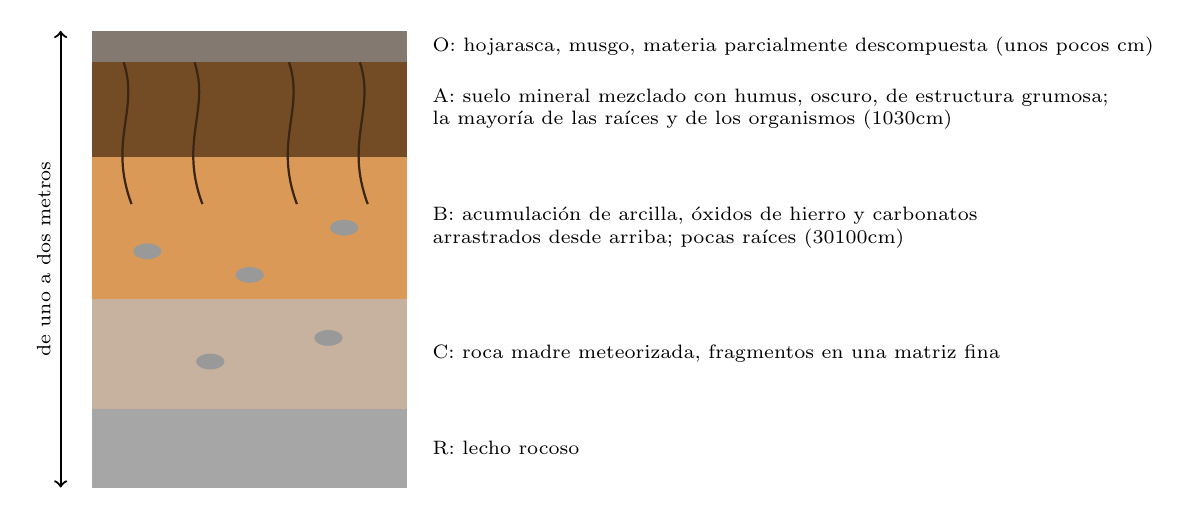
\begin{tikzpicture}[every node/.style={font=\scriptsize}]
  \fill[brown!25!black!60] (0,5.4) rectangle (4,5.8); \node[right] at (4.2,5.6) {O: hojarasca, musgo, materia parcialmente descompuesta (unos pocos cm)};
  \fill[brown!60!black] (0,4.2) rectangle (4,5.4); \node[right, align=left] at (4.2,4.8) {A: suelo mineral mezclado con humus, oscuro, de estructura grumosa;\\ la mayoría de las raíces y de los organismos (\qtyrange{10}{30}{cm})};
  \fill[brown!70!orange!80] (0,2.4) rectangle (4,4.2); \node[right, align=left] at (4.2,3.3) {B: acumulación de arcilla, óxidos de hierro y carbonatos\\ arrastrados desde arriba; pocas raíces (\qtyrange{30}{100}{cm})};
  \fill[gray!50!brown!60] (0,1.0) rectangle (4,2.4); \node[right, align=left] at (4.2,1.7) {C: roca madre meteorizada, fragmentos en una matriz fina};
  \fill[gray!70] (0,0) rectangle (4,1.0); \node[right] at (4.2,0.5) {R: lecho rocoso};
  \foreach \x in {0.4,1.3,2.5,3.4} \draw[brown!30!black, thick] (\x,5.4) .. controls (\x+0.2,4.8) and (\x-0.2,4.4) .. (\x+0.1,3.6);
  \foreach \x/\y in {0.7/3.0, 2.0/2.7, 3.2/3.3, 1.5/1.6, 3.0/1.9} \fill[gray!80] (\x,\y) ellipse (0.18 and 0.1);
  \draw[<->, thick] (-0.4,5.8) -- (-0.4,0) node[midway, left, rotate=90, anchor=south] {de uno a dos metros};
\end{tikzpicture}

{\small Un perfil de \omterm{def:b2:living-soil:soil}{suelo}. La materia orgánica entra por arriba y se
consume a medida que desciende; la materia mineral se libera en la base y
las raíces y los animales la desplazan hacia arriba; la materia disuelta
baja con el agua y queda retenida en el horizonte B.}
\end{omfigure}

\begin{proposition}[Por qué importan la arcilla y el humus]\label{prop:b2:living-soil:cec}
\index{capacidad de intercambio catiónico}\index{arcilla}\index{estructura del suelo}\index{capacidad de campo}
Las partículas de arcilla y el \omterm{def:b2:living-soil:soil}{humus} llevan cargas negativas en su
superficie y retienen, por atracción electrostática, una reserva de
cationes intercambiables ---
$\mathrm{Ca^{2+}}$, $\mathrm{Mg^{2+}}$, $\mathrm{K^{+}}$, $\mathrm{NH_4^{+}}$ --- que
las raíces aprovechan intercambiándolos por $\mathrm{H^{+}}$. Esta
\emph{\omterm{prop:b2:living-soil:cec}{capacidad de intercambio catiónico}} es el banco de nutrientes del
\omterm{def:b2:living-soil:soil}{suelo}; una arena apenas tiene (unos pocos centimoles de carga por
kilogramo), un franco arcilloso rico en \omterm{def:b2:living-soil:soil}{humus} cincuenta veces más, y la
fertilidad de ambos difiere en consecuencia. Las mismas superficies
retienen el agua: un \omterm{def:b2:living-soil:soil}{suelo} arenoso drena en un día hasta una
\emph{\omterm{prop:b2:living-soil:cec}{capacidad de campo}} de una décima parte de su volumen, un franco
retiene un tercio, y la diferencia es lo que tiene un cultivo entre dos
lluvias. Y el \omterm{def:b2:living-soil:soil}{humus}, junto con las hifas de los hongos, los exudados de
las raíces y el moco de las lombrices, pega los granos minerales en
\emph{agregados}, la estructura grumosa cuyos poros dejan pasar el aire,
el agua y las raíces --- la propiedad que distingue un \omterm{def:b2:living-soil:soil}{suelo} de un
sedimento y la primera que destruyen el arado y la compactación.
\end{proposition}

\section{Quién vive en él}

\begin{proposition}[La comunidad del suelo]\label{prop:b2:living-soil:community}
\index{red trófica del suelo}\index{detritívoro}\index{lombriz de tierra}\index{biomasa del suelo}
Un gramo de capa superficial fértil contiene unos $10^{9}$ células
bacterianas de unas diez mil especies, cien metros de hifas fúngicas,
$10^{4}$ \omterm{def:b2:unicellular-diversity:protist}{protistas}, unas decenas de nematodos y un puñado de ácaros y
colémbolos; un metro cuadrado alberga unos cientos de lombrices y, por
debajo de los animales visibles, una masa viva de varias toneladas por
hectárea --- comparable al ganado que podría mantener esa misma hectárea.
La comunidad es una \emph{red trófica detrítica}: las bacterias y los
hongos (los \emph{descomponedores}) comen materia muerta y son comidos
por \omterm{def:b2:unicellular-diversity:protist}{protistas} y nematodos (los consumidores de microorganismos), que son
comidos por ácaros y nematodos depredadores, que alimentan a ciempiés y
escarabajos; los \emph{detritívoros} --- lombrices, milpiés, cochinillas
de la humedad, termitas, colémbolos --- comen la propia hojarasca con los
microorganismos que lleva, fragmentándola mil veces y multiplicando la
superficie que atacan los microorganismos. Los consumidores de
microorganismos importan más de lo que sugiere su número: al comer
bacterias liberan en forma de amonio el nitrógeno retenido en las células
bacterianas, y un \omterm{def:b2:living-soil:soil}{suelo} con \omterm{def:b2:unicellular-diversity:protist}{protistas} y nematodos mineraliza el nitrógeno
más deprisa que uno solo con bacterias. Las lombrices son las
\emph{ingenieras del ecosistema}: sus galerías son los macroporos del
\omterm{def:b2:living-soil:soil}{suelo}, sus deyecciones son los agregados más ricos, y las lombrices de un
prado hacen pasar por su intestino unas pocas toneladas de tierra por
hectárea cada año, como midió Darwin.
\end{proposition}

\begin{omfigure}
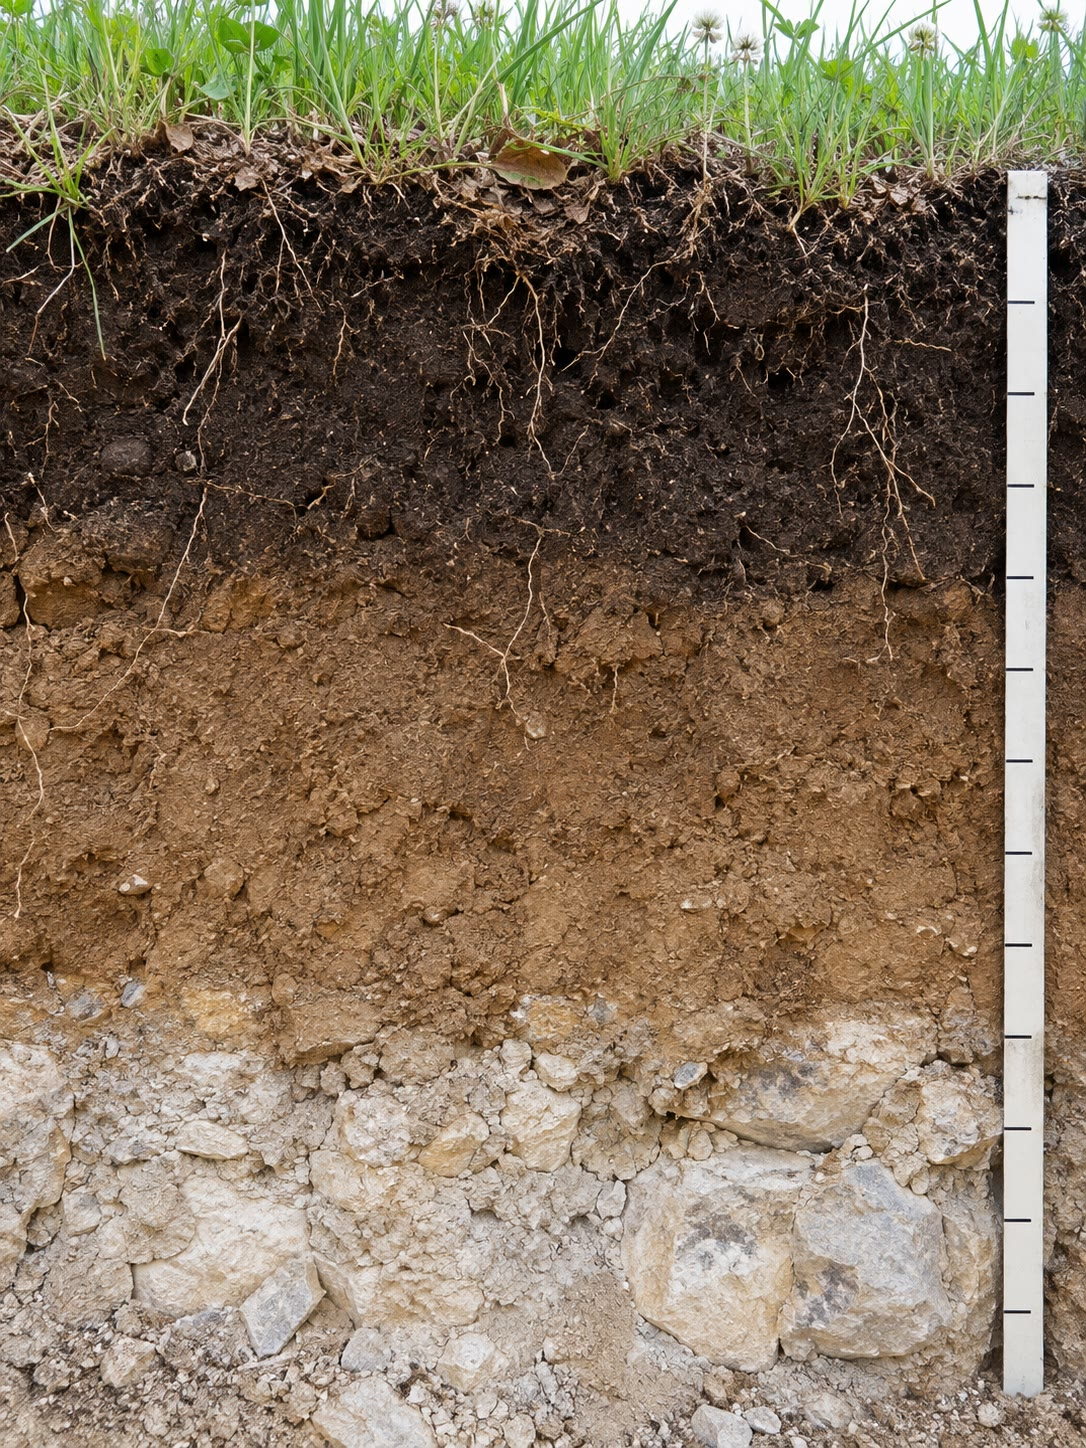
\includegraphics[width=0.21\linewidth]{images/book4/ai/b4-26-soil-profile.jpg}\hspace{0.025\linewidth}
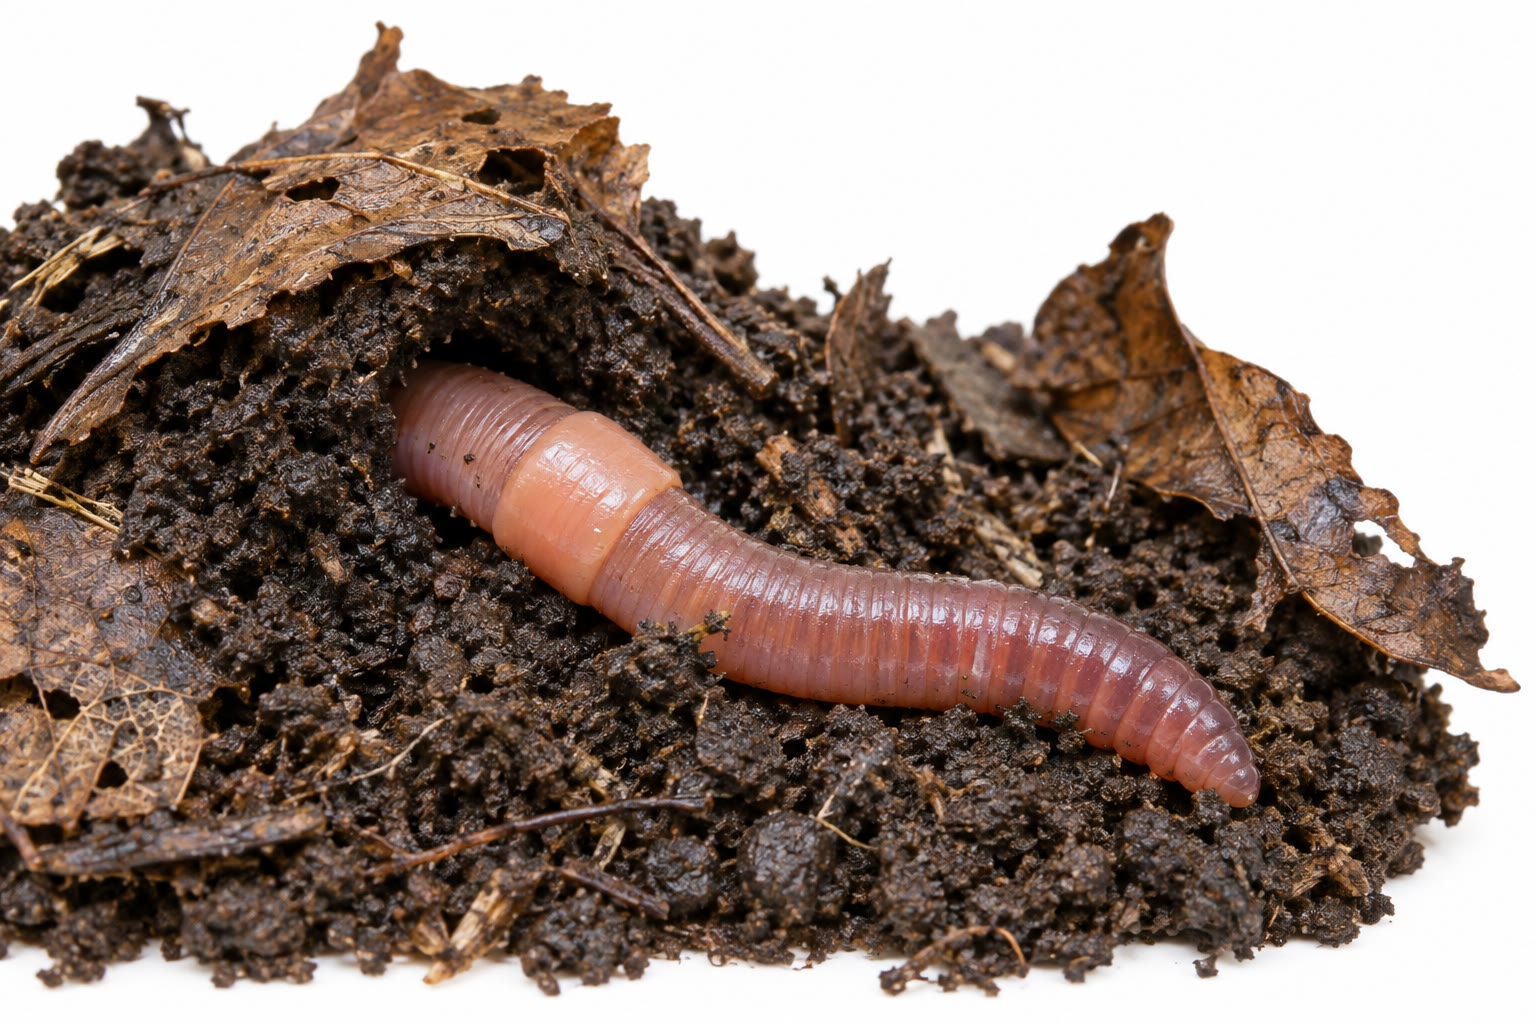
\includegraphics[width=0.42\linewidth]{images/book4/ai/b4-26-earthworm.jpg}\hspace{0.025\linewidth}
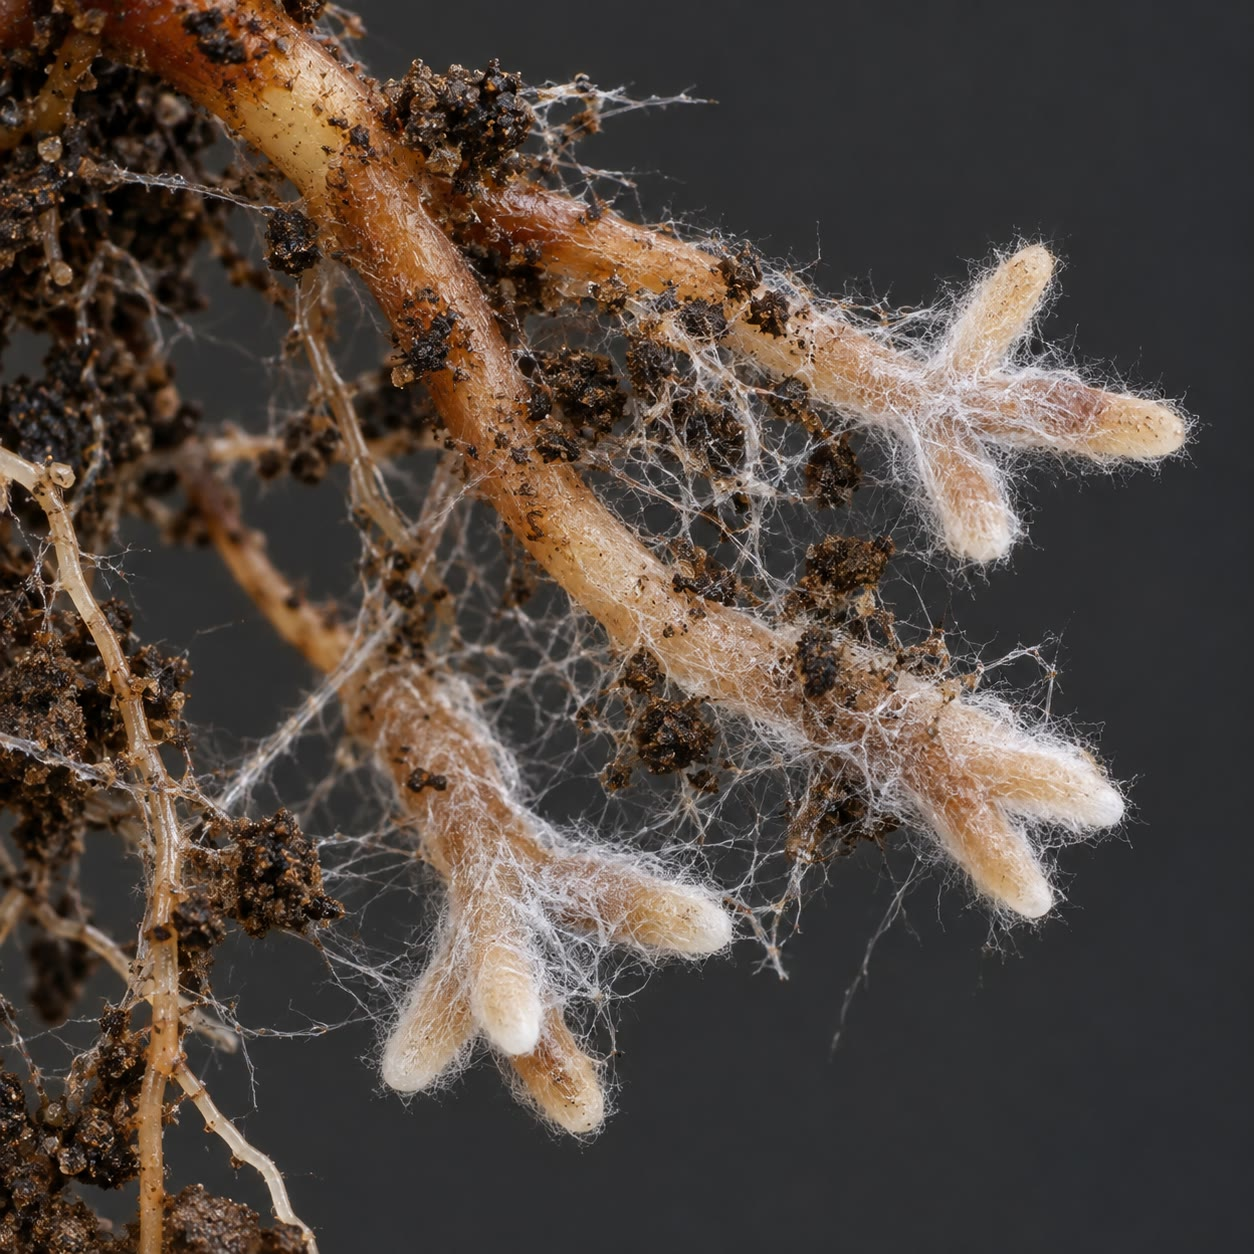
\includegraphics[width=0.28\linewidth]{images/book4/ai/b4-26-mycorrhiza.jpg}

{\small El \omterm{def:b2:living-soil:soil}{suelo} y dos de sus artífices. Izquierda: un perfil en un
talud, con la capa superficial oscura que pasa gradualmente a la roca
meteorizada clara. Centro: una lombriz en su galería. Derecha: una raíz
con su manto ectomicorrícico y las hifas que la prolongan en el \omterm{def:b2:living-soil:soil}{suelo}.}
\end{omfigure}

\section{La descomposición}

\begin{theorem}[La descomposición de la hojarasca y el cociente carbono/nitrógeno]\label{thm:b2:living-soil:decay}
\index{descomposición}\index{descomposición de la hojarasca}\index{cociente C:N}\index{mineralización}\index{inmovilización}
La hojarasca se descompone a una velocidad proporcional a lo que queda,
$\mathrm{d}L/\mathrm{d}t = -kL$, de modo que $L = L_0 e^{-kt}$, con una
\emph{constante de descomposición} $k$ de alrededor de 1 por año para la
hierba y las hojas caducas de un bosque templado, $0.3$ para las acículas
de las coníferas, varias por año en los trópicos húmedos y $0.05$ en la
tundra; un aporte constante $I$ por año forma una capa de hojarasca de
$I/k$. La descomposición depende de la temperatura, de la humedad y de la
\emph{calidad} de la hojarasca: su contenido en nitrógeno, su contenido en
lignina y el cociente entre carbono y nitrógeno. Los microorganismos
tienen $\mathrm{C:N} \approx 8$ y retienen alrededor del \qty{40}{\%} del
carbono que comen, de modo que necesitan un nitrógeno por cada
$8/0.4 = 20$ carbonos de alimento: la hojarasca con un $\mathrm{C:N}$
inferior a unos 25 libera amonio al descomponerse
(\emph{mineralización}), mientras que la que lo supera --- la paja, con
80; la \omterm{def:b2:plant-meristems:wood}{madera}, con 400 --- obliga a los microorganismos a tomar nitrógeno
del \omterm{def:b2:living-soil:soil}{suelo} (\emph{inmovilización}), privando de él a las plantas hasta que
el carbono se ha respirado y el cociente ha bajado. Por eso la paja fresca
enterrada con el arado perjudica a un cultivo, por eso los restos de
leguminosas lo alimentan, y por eso un montón de compost necesita ambos.
\end{theorem}
\begin{proof}
Para el cociente: los microorganismos que comen hojarasca con $c$ carbonos
por nitrógeno asimilan $0.4c$ carbonos y, para formar biomasa con
$\mathrm{C:N} = 8$, necesitan $0.4c/8 = c/20$ nitrógenos; la hojarasca
aporta 1. Si $c < 20$, sobra nitrógeno, que se libera como amonio; si
$c > 20$, hay un déficit que se toma del \omterm{def:b2:living-soil:soil}{suelo}. El umbral de 25 que se
observa en la práctica refleja una eficiencia de retención algo inferior a
0,4. Para la capa de hojarasca: $\mathrm{d}L/\mathrm{d}t = I - kL$
tiene como \omterm{def:b2:biogeochemical-cycles:reservoir}{estado estacionario} $I/k$, al que se aproxima con una constante
de tiempo $1/k$; el \omterm{def:b2:biogeochemical-cycles:reservoir}{tiempo de residencia} de la hojarasca es $1/k$, un año
en un hayedo y veinte en la tundra.
\end{proof}
\begin{proof}[Evidencia]
Los experimentos con bolsas de hojarasca --- masas conocidas de hojas en
bolsas de malla, enterradas y pesadas a intervalos --- dieron la ley
exponencial y sus constantes en todos los biomas (Olson, 1963), y
mostraron, con distintos tamaños de malla, que excluir a los animales del
\omterm{def:b2:living-soil:soil}{suelo} reduce a la mitad la velocidad: los microorganismos hacen la química,
pero los animales marcan el ritmo. A escala de un continente, la misma
hoja se descompone en un año en Georgia y en ocho en Alaska, en proporción
a la evapotranspiración real, el producto del calor y del agua.
\end{proof}

\begin{omfigure}
\begin{tikzpicture}
\begin{axis}[
  width=0.72\linewidth, height=5.6cm,
  axis x line=bottom, axis y line=left,
  xmin=0, xmax=6, ymin=0, ymax=105,
  xlabel={años}, ylabel={masa de hojarasca restante (\%)},
  xlabel style={font=\small, at={(axis description cs:0.5,-0.13)}, anchor=north},
  ylabel style={font=\small},
  tick label style={font=\small},
  legend style={font=\scriptsize, at={(0.5,-0.3)}, anchor=north, draw=none, legend columns=2},
  clip=false,
]
\addplot[very thick, omDef, domain=0:6, samples=60] {100*exp(-2*x)};
\addlegendentry{hoja de bosque tropical, $k = 2$}
\addplot[very thick, omThm, domain=0:6, samples=60] {100*exp(-1*x)};
\addlegendentry{hoja de haya, $k = 1$}
\addplot[very thick, omProp, domain=0:6, samples=60] {100*exp(-0.3*x)};
\addlegendentry{acícula de pícea, $k = 0.3$}
\addplot[very thick, gray, domain=0:6, samples=60] {100*exp(-0.05*x)};
\addlegendentry{musgo de tundra, $k = 0.05$}
\end{axis}
\end{tikzpicture}

{\small Descomposición exponencial de la hojarasca. La mitad de una hoja de
haya desaparece en ocho meses; la mitad de un \omterm{def:b2:plant-life-cycles:moss}{musgo} de tundra, en catorce
años; el residuo que ni los microorganismos ni los animales pueden
terminar se convierte en \omterm{def:b2:living-soil:soil}{humus}.}
\end{omfigure}

\begin{proposition}[El humus y la reserva de carbono del suelo]\label{prop:b2:living-soil:humus}
\index{humus}\index{carbono orgánico del suelo}\index{respiración del suelo}
Un pequeño porcentaje del carbono de la hojarasca escapa a la oxidación
completa y se convierte en \emph{\omterm{def:b2:living-soil:soil}{humus}}: una mezcla oscura y amorfa de
residuos microbianos, lignina alterada y compuestos vegetales, unida a la
arcilla y al hierro y encerrada en los agregados, que se descompone con
\omterm{def:b2:biogeochemical-cycles:reservoir}{tiempos de residencia} de décadas a milenios. En el \omterm{def:b2:living-soil:soil}{humus} reside la
fertilidad del \omterm{def:b2:living-soil:soil}{suelo}
--- la mayor parte de su nitrógeno y de su intercambio catiónico, la mitad
de su capacidad de retener agua --- y es la mayor reserva de carbono
orgánico de las tierras emergidas,
\qty{1700}{GtC} en el primer metro, el doble que la atmósfera. Su
balance es el aporte menos la descomposición, $\mathrm{d}H/\mathrm{d}t = I_h - k_hH$:
con $k_h \approx 0.02$ por año, un \omterm{def:b2:living-soil:soil}{suelo} contiene cincuenta años de aporte,
y cualquier cambio --- el arado, que rompe los agregados y airea el \omterm{def:b2:living-soil:soil}{humus};
el drenaje de una turbera, que deja entrar el oxígeno; el calentamiento,
que eleva $k_h$ --- se manifiesta como una pérdida que continúa durante
décadas. Los \omterm{def:b2:living-soil:soil}{suelos} cultivados del mundo han perdido entre un tercio y la
mitad de su \omterm{def:b2:living-soil:soil}{humus} desde que se roturaron por primera vez, unas
\qty{100}{GtC}, y un calentamiento de \qty{3}{\celsius} aumentaría en un
tercio la descomposición del resto: los \omterm{def:b2:living-soil:soil}{suelos} son la mayor incertidumbre
del balance de carbono del \cref{ch:b2:global-change}.
\end{proposition}

\section{Asociaciones bajo tierra}

\begin{proposition}[Micorrizas y rizobios]\label{prop:b2:living-soil:symbiosis}
\index{micorriza}\index{rizobio}\index{nódulo radical}\index{nitrogenasa}\index{leghemoglobina}
Nueve especies de plantas de cada diez tienen las raíces colonizadas por
hongos en una \emph{micorriza}: la planta da azúcar (entre una décima y una
quinta parte de sus fotosintatos) y el hongo da fosfato, nitrógeno, agua y
cinc, que sus hifas, cien veces más finas que una raíz y cien veces más
largas por unidad de carbono, recogen de un volumen de \omterm{def:b2:living-soil:soil}{suelo} que la raíz
no puede alcanzar --- sobre todo el fosfato, que difunde tan despacio por
el \omterm{def:b2:living-soil:soil}{suelo} que una raíz agota en unos días el milímetro que la rodea. Las
micorrizas \emph{arbusculares}, el tipo más antiguo, penetran en las
células de la raíz y se ramifican en arbúsculos, donde tiene lugar el
intercambio; las \emph{ectomicorrizas} de los árboles forestales envuelven
el ápice de la raíz y crecen entre sus células. Las leguminosas van más
lejos: los rizobios, atraídos por los flavonoides de la raíz, entran por un
pelo radical, y la raíz construye a su alrededor un \emph{nódulo} en el que
las bacterias, convertidas en \emph{bacteroides}, fijan nitrógeno con la
nitrogenasa --- una enzima tan sensible al oxígeno que el nódulo debe
mantenerse casi anóxico gracias a la \emph{leghemoglobina}, una
hemoglobina que fabrica la planta, que da al nódulo su color rosado y
entrega el oxígeno a los bacteroides a una concentración demasiado baja
para envenenar la enzima. Cada socio vigila al otro: una planta corta el
azúcar a los nódulos que no fijan nada, y un hongo que entrega menos
fosfato recibe menos carbono.
\end{proposition}
\begin{proof}[Evidencia]
Kiers y sus colaboradores (2011) cultivaron una planta con dos hongos
asociados sobre un sistema radical dividido y ofrecieron fosfato a un solo
lado: la planta asignaba más carbono al hongo que aportaba más fosfato, y
el hongo asignaba más fosfato a la raíz que daba más carbono --- recompensas
recíprocas medidas con isótopos. En el caso de los rizobios, los nódulos a
los que se impidió experimentalmente obtener nitrógeno (sustituyendo el
aire por argón y oxígeno) recibían menos oxígeno y crecían menos que los
nódulos de la misma planta que podían fijar: la planta sanciona a los
tramposos. El marcaje con nitrógeno 15 muestra que un prado de trébol y
gramíneas transfiere a las gramíneas un tercio del nitrógeno fijado por el
trébol en una sola estación, a través del \omterm{def:b2:living-soil:soil}{suelo} y de redes fúngicas
compartidas.
\end{proof}

\begin{omfigure}
\begin{tikzpicture}[every node/.style={font=\scriptsize}, >=stealth]
  % root cross-section
  \fill[omThm!15] (0,0) circle (1.5); \draw[thick] (0,0) circle (1.5);
  \fill[omThm!30] (0,0) circle (0.5); \draw[thick] (0,0) circle (0.5);
  \node at (0,0) {estela};
  \node at (0,1.05) {córtex};
  % arbuscules in cortex cells
  \foreach \a in {30,150,270} { \draw[omDef, thick] ({1.0*cos(\a)},{1.0*sin(\a)}) -- ++({0.25*cos(\a+60)},{0.25*sin(\a+60)}) -- ++({0.2*cos(\a-40)},{0.2*sin(\a-40)}); \draw[omDef, thick] ({1.0*cos(\a)},{1.0*sin(\a)}) -- ++({0.25*cos(\a-60)},{0.25*sin(\a-60)}); }
  % hyphae out
  \foreach \a in {20,80,150,210,340} { \draw[omDef, thick] ({1.5*cos(\a)},{1.5*sin(\a)}) .. controls ({2.2*cos(\a+10)},{2.2*sin(\a+10)}) .. ({2.7*cos(\a-5)},{2.7*sin(\a-5)}); }
  \draw[omDef, thick] ({1.5*cos(150)},{1.5*sin(150)}) -- ({1.0*cos(150)},{1.0*sin(150)});
  \node[omDef, anchor=west, align=left] at (2.9,1.4) {hifas: \qty{3}{\micro m} de ancho,\\ metros por centímetro de raíz};
  \node[omDef, anchor=west] at (2.9,0.1) {arbúsculo dentro de una célula del córtex};
  \draw[omDef] (2.85,0.1) -- (1.2,0.5);
  \node[anchor=north, align=center] at (0,-1.6) {raíz, \qty{0.3}{mm} de diámetro};
  \draw[->, thick, omThm] (-1.2,-2.4) -- (1.2,-2.4) node[right] {azúcar hacia el hongo, \qtyrange{10}{20}{\%} de los fotosintatos};
  \draw[<-, thick, omDef] (-1.2,-2.9) -- (1.2,-2.9) node[right] {fosfato, amonio, agua y cinc hacia la planta};
  % nodule
  \begin{scope}[xshift=9.3cm]
    \draw[thick, brown!60!black] (-0.3,2.4) -- (-0.1,-0.6);
    \draw[thick, brown!60!black] (-0.1,0.3) -- (1.6,0.1);
    \fill[pink!60!red!40] (1.5,0.2) circle (0.9); \draw[thick] (1.5,0.2) circle (0.9);
    \fill[pink!80!red!60] (1.5,0.2) circle (0.55);
    \foreach \p in {(1.3,0.3),(1.6,0.0),(1.5,0.45),(1.7,0.3),(1.35,0.05)} \fill[omDef!70!black] \p ellipse (0.08 and 0.05);
    \node[anchor=north, align=center] at (1.5,-0.8) {nódulo: bacteroides en células vegetales,\\ rosado por la leghemoglobina;\\ oxígeno mantenido a \qty{10}{nM}: la nitrogenasa\\ funciona y las células siguen respirando};
    \node[anchor=south, align=center] at (-0.2,2.45) {raíz de leguminosa};
  \end{scope}
\end{tikzpicture}

{\small Dos pactos. Izquierda: una micorriza arbuscular, con el azúcar que
sale y el fosfato que entra a través de los arbúsculos situados dentro de
las células del córtex. Derecha: un nódulo de leguminosa, donde la propia
hemoglobina de la planta mantiene el oxígeno lo bastante bajo para la
nitrogenasa y lo bastante alto para la respiración.}
\end{omfigure}

\section{Perder el suelo}

\begin{proposition}[La erosión, la sal y el balance de un suelo]\label{prop:b2:living-soil:erosion}
\index{erosión del suelo}\index{salinización}\index{desertificación}
El \omterm{def:b2:living-soil:soil}{suelo} se forma a razón de \qtyrange{0.05}{0.5}{mm} al año y, bajo la
vegetación natural, se erosiona aproximadamente al mismo ritmo. Una tierra
desnuda y arada en pendiente pierde \qtyrange{1}{10}{mm} al año por el
agua y el viento ---
\qtyrange{10}{100}{t/ha} ---, de diez a cien veces el ritmo de formación:
un \omterm{def:b2:living-soil:soil}{suelo} formado en diez mil años desaparece en un siglo, y con él el
\omterm{def:b2:living-soil:soil}{humus} y los nutrientes del horizonte A, la única parte que importa. Los
cultivos de cobertura, las terrazas, el arado siguiendo las curvas de
nivel y el cultivo sin labranza, que deja los restos en la superficie y
los agregados intactos, devuelven la pérdida a un valor cercano al ritmo
de formación. El riego en climas secos provoca el fallo opuesto: el agua
se evapora y deja sus sales, una tonelada por hectárea al año a partir de
un agua que solo es ligeramente salina, hasta que el potencial osmótico de
la solución del \omterm{def:b2:living-soil:soil}{suelo} (\cref{ch:b2:plant-plasticity}) es más bajo de lo que
las raíces pueden superar --- la \emph{salinización}, que dejó
improductivos los campos de Sumer hace cuatro mil años y afecta hoy a una
quinta parte de las tierras de regadío. El estado de un \omterm{def:b2:living-soil:soil}{suelo} es un
balance: \omterm{def:b2:living-soil:soil}{humus} que entra frente a \omterm{def:b2:living-soil:soil}{humus} que sale, formación frente a
erosión, sal que entra frente a sal drenada; cada término tiene un \omterm{def:b2:biogeochemical-cycles:reservoir}{tiempo
de residencia}, y cada uno, una vez negativo, tarda en invertirse.
\end{proposition}

\section{Ejercicios}

\begin{exercise}[$\star$]\label{exo:b2:living-soil:1}
Nómbrense los horizontes de un perfil de \omterm{def:b2:living-soil:soil}{suelo} desde la superficie hacia
abajo e indíquese qué ocurre en cada uno.
\end{exercise}

\begin{exercise}[$\star$]\label{exo:b2:living-soil:2}
Explíquese qué es la \omterm{prop:b2:living-soil:cec}{capacidad de intercambio catiónico}, por qué un \omterm{def:b2:living-soil:soil}{suelo}
arenoso tiene poca y qué le hace a un \omterm{def:b2:living-soil:soil}{suelo} ácido el agricultor que lo
encala.
\end{exercise}

\begin{exercise}[$\star$]\label{exo:b2:living-soil:3}
Enumérense los principales grupos de la \omterm{prop:b2:living-soil:community}{red trófica del suelo}, desde los
descomponedores hasta los superdepredadores, con un organismo de cada uno,
e indíquese qué hacen por las plantas los consumidores de bacterias.
\end{exercise}

\begin{exercise}[$\star$]\label{exo:b2:living-soil:4}
Distíngase entre micorrizas arbusculares y ectomicorrizas, e indíquese qué
da y qué recibe cada socio.
\end{exercise}

\begin{exercise}[$\star\star$]\label{exo:b2:living-soil:5}
Un hayedo deja caer \qty{4}{t/ha} de hojas al año y su hojarasca se
descompone con $k = 0.8$ por año. Calcúlense la masa de hojarasca en
\omterm{def:b2:biogeochemical-cycles:reservoir}{estado estacionario}, el \omterm{def:b2:biogeochemical-cycles:reservoir}{tiempo de residencia} de la hojarasca y el tiempo
que tarda la caída de un año en perder el \qty{90}{\%} de su masa.
\end{exercise}

\begin{exercise}[$\star\star$]\label{exo:b2:living-soil:6}
La paja de trigo tiene $\mathrm{C:N} = 80$ y los restos de trébol $15$. Para
cada uno, calcúlense el nitrógeno que necesitan los microorganismos por
cada \qty{100}{kg} de carbono consumido (retención de 0,4, microorganismos con
$\mathrm{C:N} = 8$) y si el resto mineraliza o inmoviliza nitrógeno, y
cuánto.
\end{exercise}

\begin{exercise}[$\star\star$]\label{exo:b2:living-soil:7}
Una hectárea de prado contiene \qty{2}{t} de lombrices, cada una de las
cuales procesa al año diez veces su masa en tierra. Calcúlense la tierra
que pasa por las lombrices cada año y el tiempo que tardan los
\qty{20}{cm} superiores (densidad aparente de \qty{1.3}{t/m^3}) en pasar
una vez. Compárese con la cifra de Darwin.
\end{exercise}

\begin{exercise}[$\star\star$]\label{exo:b2:living-soil:8}
Un gramo de \omterm{def:b2:living-soil:soil}{suelo} contiene $10^{9}$ bacterias de \qty{e-12}{g} cada una, y
\qty{100}{m} de hifas de \qty{4}{\micro m} de diámetro y
\qty{1.1}{g/cm^3} de densidad. Calcúlense la biomasa bacteriana y la
fúngica por gramo y por hectárea (\qty{20}{cm} superiores,
\qty{1.3}{t/m^3}).
\end{exercise}

\begin{exercise}[$\star\star$]\label{exo:b2:living-soil:9}
El \omterm{def:b2:living-soil:soil}{humus} del \omterm{def:b2:living-soil:soil}{suelo} se descompone con $k_h = 0.02$ por año y recibe
\qty{1.5}{t/ha} de carbono al año. Calcúlese el carbono del \omterm{def:b2:living-soil:soil}{humus} en
\omterm{def:b2:biogeochemical-cycles:reservoir}{estado estacionario}. El campo se ara y $k_h$ se duplica: calcúlense el nuevo
\omterm{def:b2:biogeochemical-cycles:reservoir}{estado estacionario}, el carbono perdido y el tiempo que se tarda en perder
la mitad.
\end{exercise}

\begin{exercise}[$\star\star\star$]\label{exo:b2:living-soil:10}
El fosfato difunde por el \omterm{def:b2:living-soil:soil}{suelo} con $D \approx \qty{e-13}{m^2/s}$.
Calcúlese la distancia que recorre en una temporada de crecimiento de
\num{100} días ($x \approx \sqrt{2Dt}$) y compárese con la separación
entre raíces (\qty{1}{cm}) y entre hifas (\qty{0.1}{mm}). ¿Qué dice esto
sobre por qué las micorrizas importan para el fósforo y menos para el
nitrato
($D \approx \qty{e-10}{m^2/s}$)?
\end{exercise}

\begin{exercise}[$\star\star\star$]\label{exo:b2:living-soil:11}
Una ladera pierde \qty{20}{t/ha} de \omterm{def:b2:living-soil:soil}{suelo} al año por erosión mientras
forma \qty{1}{t/ha}; el horizonte A tiene \qty{25}{cm} de espesor, a
\qty{1.3}{t/m^3}, y contiene un \qty{3}{\%} de carbono. Calcúlense la masa
del horizonte A, su duración a este ritmo y el carbono perdido por año.
Sin labranza, la pérdida baja a \qty{2}{t/ha}: vuélvase a calcular la
duración.
\end{exercise}

\begin{exercise}[$\star\star\star$]\label{exo:b2:living-soil:12}
``El \omterm{def:b2:living-soil:soil}{suelo} es el organismo más lento de la granja.'' Discútase con los
\omterm{def:b2:biogeochemical-cycles:reservoir}{tiempos de residencia} de la hojarasca, el \omterm{def:b2:living-soil:soil}{humus}, el \omterm{def:b2:living-soil:soil}{suelo} mineral y la sal,
e indíquese qué cambios puede ver un agricultor a lo largo de su vida
profesional y cuáles no.
\end{exercise}

\section{Problema: una hectárea de suelo}

\begin{problem}[{Problema de fin de semana --- una hectárea de suelo de
cultivo auditada: su masa viva contada, su hojarasca y su humus seguidos a
través de sus balances exponenciales, el nitrógeno liberado por unos
restos de leguminosa calculado frente a las necesidades de un cultivo, y
las cuentas de erosión y de carbono de dos sistemas de manejo comparadas,
hasta llegar a la reserva de carbono del suelo, su duración bajo el arado
y el nitrógeno que aporta una leguminosa}]
\label{pb:b2:living-soil:1}
La hectárea: horizonte A de \qty{25}{cm} de espesor, densidad aparente de
\qty{1.3}{t/m^3}, \qty{2.5}{\%} de carbono orgánico; descomposición del
\omterm{def:b2:living-soil:soil}{humus} $k_h =
0.025$ por año con arado, $0.015$ sin labranza; aporte de carbono al \omterm{def:b2:living-soil:soil}{humus}
de \qty{1.2}{t/ha} al año en ambos casos. Hojarasca: un cultivo de
cobertura de trébol deja \qty{5}{t/ha} de materia seca con un
\qty{45}{\%} de carbono y un \qty{3}{\%} de nitrógeno, que se descompone
con $k = 2$ por año. Erosión: \qty{15}{t/ha} al año con arado,
\qty{1.5}{t/ha} sin labranza; formación de \qty{0.5}{t/ha}.

\medskip
\noindent\textbf{Parte I --- La reserva.}
\begin{enumerate}
  \item Calcúlense la masa del horizonte A y su carbono orgánico.
  \item Calcúlese la masa de nitrógeno del \omterm{def:b2:living-soil:soil}{humus} si su
        $\mathrm{C:N}$ es 12.
  \item El \omterm{def:b2:living-soil:soil}{suelo} contiene $10^{9}$ bacterias por gramo, de \qty{e-12}{g}
        cada una, y \qty{200}{m} de hifas por gramo, de \qty{4}{\micro m}
        de diámetro y densidad 1,1. Calcúlese la biomasa microbiana por
        hectárea.
  \item Añádanse \qty{1.5}{t/ha} de lombrices y \qty{0.2}{t/ha} de otros
        animales, y dese la masa viva total por hectárea. ¿Qué fracción
        representa del carbono del \omterm{def:b2:living-soil:soil}{humus}?
  \item Los microorganismos renuevan su biomasa dos veces al año y
        respiran el \qty{60}{\%} de lo que comen. Estímense el carbono que
        consumen al año y el $\mathrm{CO_2}$ respirado.
  \item Compárese con la producción primaria neta del cultivo, de unas
        \qty{5}{t/ha} de carbono, y coméntese.
\end{enumerate}

\medskip
\noindent\textbf{Parte II --- Los restos de trébol.}
\begin{enumerate}[resume]
  \item Calcúlense el carbono y el nitrógeno de los restos y su
        $\mathrm{C:N}$.
  \item Con microorganismos de $\mathrm{C:N} = 8$ y una retención de $0.4$,
        ¿mineralizan o inmovilizan nitrógeno los restos? Calcúlese el
        nitrógeno neto liberado cuando se descomponen por completo.
  \item Con $k = 2$, ¿qué fracción de los restos se ha descompuesto al cabo
        de 3 meses? ¿Y al cabo de un año?
  \item Calcúlese el nitrógeno liberado en los 3 primeros meses.
  \item Un cultivo de trigo absorbe \qty{150}{kg} de nitrógeno por
        hectárea, la mayor parte en los dos meses siguientes a la siembra.
        Coméntese el calendario.
  \item En su lugar se entierra la misma masa de paja de trigo
        ($\mathrm{C:N} = 80$). Calcúlese el nitrógeno inmovilizado e
        indíquese qué debe hacer el agricultor.
\end{enumerate}

\medskip
\noindent\textbf{Parte III --- El \omterm{def:b2:living-soil:soil}{humus}.}
\begin{enumerate}[resume]
  \item Calcúlese el carbono del \omterm{def:b2:living-soil:soil}{humus} en \omterm{def:b2:biogeochemical-cycles:reservoir}{estado estacionario} con arado y
        sin labranza.
  \item El campo, en el \omterm{def:b2:biogeochemical-cycles:reservoir}{estado estacionario} con arado, pasa al cultivo sin
        labranza. Escríbase $H(t)$ y calcúlese el carbono ganado al cabo de
        10 y de 50 años.
  \item Calcúlese la velocidad de ganancia el primer año, en toneladas de
        carbono por hectárea y en toneladas de $\mathrm{CO_2}$.
  \item Si las \qty{1.5e9}{ha} de tierras de cultivo del mundo hicieran lo
        mismo, ¿cuál sería el sumidero el primer año, frente a unas
        emisiones fósiles de \qty{10}{GtC}? ¿Y el quincuagésimo año?
  \item ¿Por qué el sumidero es temporal y reversible?
  \item Un calentamiento de \qty{3}{\celsius} aumenta $k_h$ en un tercio.
        Calcúlense el nuevo \omterm{def:b2:biogeochemical-cycles:reservoir}{estado estacionario} sin labranza y el carbono
        perdido.
\end{enumerate}

\medskip
\noindent\textbf{Parte IV --- La erosión.}
\begin{enumerate}[resume]
  \item Calcúlese la pérdida neta de \omterm{def:b2:living-soil:soil}{suelo} por año con cada sistema.
  \item Calcúlese la duración del horizonte A con cada uno.
  \item Calcúlense el carbono y el nitrógeno que arrastra la erosión cada
        año con arado.
  \item Compárese la pérdida de carbono por erosión con la pérdida por
        descomposición del \omterm{def:b2:living-soil:soil}{humus} en el \omterm{def:b2:biogeochemical-cycles:reservoir}{estado estacionario} con arado.
  \item El \omterm{def:b2:living-soil:soil}{suelo} erosionado se deposita aguas abajo. ¿Se pierde su carbono
        hacia la atmósfera? Discútase.
  \item Dense los \omterm{def:b2:biogeochemical-cycles:reservoir}{tiempos de residencia} de la hojarasca, el \omterm{def:b2:living-soil:soil}{humus} y el \omterm{def:b2:living-soil:soil}{suelo}
        mineral en esta hectárea.
  \item Enúnciese el resultado: la reserva de carbono del horizonte A, su
        duración con arado y sin labranza, y el nitrógeno que aportan los
        restos de trébol.
\end{enumerate}
\end{problem}
